\section{Introduction and Background}

\subsection{Climate Change and Heat-Health Impacts in the Johannesburg Context}

Climate change has intensified heat-related health risks in Johannesburg, where rising temperatures are linked to increasing mortality and morbidity \citep{Gasparrini2015, Romanello2023}. With over 5.87 million inhabitants, the city faces substantial warming projections—by 2050, mean temperatures may rise approximately 2°C with hot nights projected to quadruple \citep{Engelbrecht2015, WorldBank2024}. Current research indicates that above 18.7°C apparent temperature, all-cause mortality rises by 0.9\% per 1°C increase, with seniors experiencing 2.1\% increases \citep{Wichmann2017}. The IPCC warns that beyond +2°C of global warming, heat-attributable health impacts in Africa will sharply rise \citep{IPCC2024}.

\subsection{Socio-Spatial Inequity and Heat Vulnerability}

Johannesburg's socio-spatial layout—largely a legacy of apartheid-era planning—significantly shapes contemporary heat vulnerability patterns. Historical policies created wealthy suburbs with green spaces alongside dense townships with minimal vegetation, resulting in temperature differentials of approximately 6°C between affluent neighborhoods and informal settlements \citep{WorldBank2024}. Housing quality further exacerbates this disparity, with informal dwellings experiencing up to 15°C higher indoor temperatures than formal housing \citep{Naicker2017}. This embedded vulnerability continues to cluster heat-health risks in historically marginalized communities \citep{Strauss2019}.

\subsection{Research Context and Positionality}
This research builds upon ongoing work at the HE²AT Center, which has established baseline heat vulnerability assessment frameworks for South African cities \citep{Jack}. As a researcher within this initiative, I bring expertise in data science and machine learning methods to extend these frameworks through advanced statistical techniques. My position at the intersection of public health and climate science informs a multidisciplinary approach that aims to translate complex data into actionable health interventions. This work specifically addresses gaps in the Heat Center's existing vulnerability assessments by developing dynamic predictive models that can account for temporal changes in vulnerability patterns across Johannesburg's diverse socioeconomic landscape.

\subsection{Conceptual Framework and Research Gaps}

This research employs a comprehensive framework for heat vulnerability encompassing three interconnected dimensions: exposure, sensitivity, and adaptive capacity \citep{IPCC2022}. Figure \ref{fig:conceptual_framework} illustrates these relationships and their determinants within Johannesburg's urban context.

\begin{figure}[h]
\centering
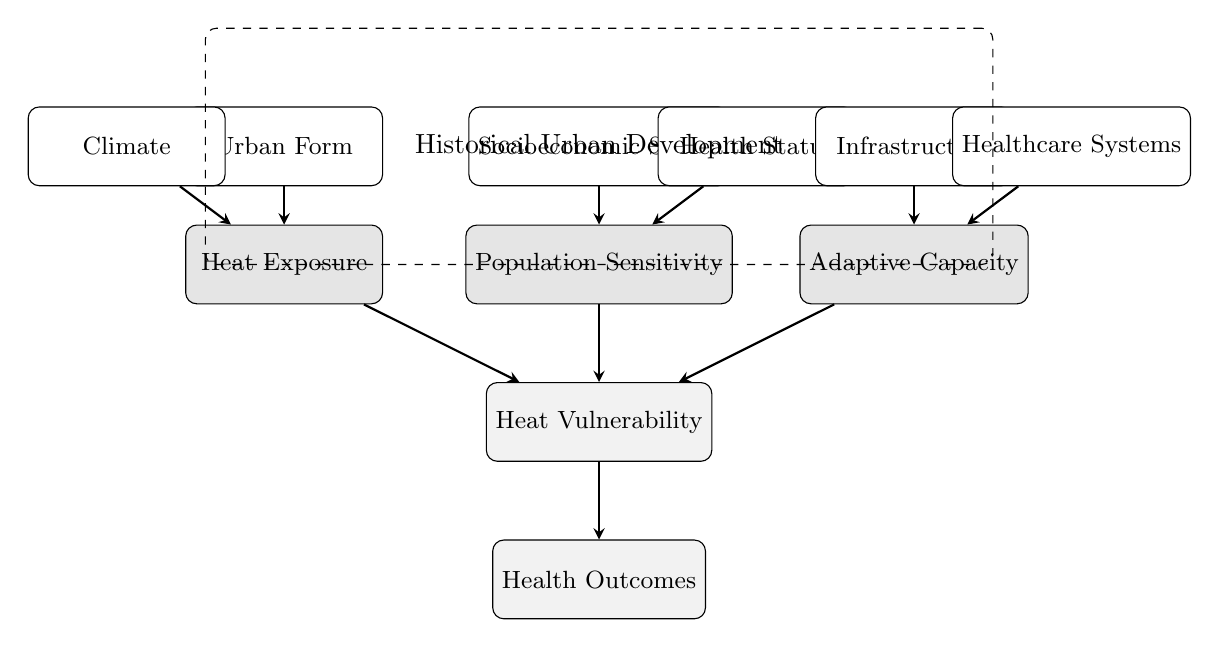
\begin{tikzpicture}[
    node distance=1.5cm,
    box/.style={rectangle, draw, rounded corners, minimum width=2.5cm, minimum height=1cm, text centered, font=\small},
    arrow/.style={thick, ->, >=stealth}
]

% Main components
\node[box, fill=gray!20] (exposure) at (0,0) {Heat Exposure};
\node[box, fill=gray!20] (sensitivity) at (4,0) {Population Sensitivity};
\node[box, fill=gray!20] (adaptive) at (8,0) {Adaptive Capacity};
\node[box, fill=gray!10] (vulnerability) at (4,-2) {Heat Vulnerability};
\node[box, fill=gray!10] (outcomes) at (4,-4) {Health Outcomes};

% Environmental factors
\node[box, fill=white] (urban) at (0,1.5) {Urban Form};
\node[box, fill=white] (climate) at (-2,1.5) {Climate};

% Socioeconomic factors
\node[box, fill=white] (socio) at (4,1.5) {Socioeconomic Status};
\node[box, fill=white] (health) at (6,1.5) {Health Status};

% Adaptation factors
\node[box, fill=white] (infra) at (8,1.5) {Infrastructure};
\node[box, fill=white] (systems) at (10,1.5) {Healthcare Systems};

% Connections
\draw[arrow] (exposure) -- (vulnerability);
\draw[arrow] (sensitivity) -- (vulnerability);
\draw[arrow] (adaptive) -- (vulnerability);
\draw[arrow] (vulnerability) -- (outcomes);

% Environmental connections
\draw[arrow] (climate) -- (exposure);
\draw[arrow] (urban) -- (exposure);

% Socioeconomic connections
\draw[arrow] (socio) -- (sensitivity);
\draw[arrow] (health) -- (sensitivity);

% Adaptation connections
\draw[arrow] (infra) -- (adaptive);
\draw[arrow] (systems) -- (adaptive);

% Historical influence
\node[draw, dashed, rounded corners, minimum width=10cm, minimum height=3cm] at (4,1.5) {Historical Urban Development};

\end{tikzpicture}
\caption{Conceptual framework of heat vulnerability in Johannesburg, highlighting the three primary dimensions (exposure, sensitivity, adaptive capacity) and their determinants. The dashed outline indicates components influenced by historical urban development patterns including apartheid-era planning.}
\label{fig:conceptual_framework}
\end{figure}

These components interact as follows:
\begin{itemize}
    \item \textit{Exposure} refers to heat stress degree and duration, with dense urban areas showing significantly higher surface temperatures (up to 5\textdegree C) compared to well-vegetated neighbourhoods \citep{Li2017, Santamouris2015}.
    
    \item \textit{Sensitivity} reflects population susceptibility influenced by socio-economic conditions and health status, with chronic conditions significantly increasing heat-related health risks \citep{Watts2023, Khosla2021, Souverijns2022}.
    
    \item \textit{Adaptive capacity} depends on access to healthcare, cooling infrastructure, and social support systems \citep{Ansah2024}, with limited access to healthcare affecting vulnerability to heat, as demonstrated by increased heat-related mortality in areas with restricted medical services \citep{Murage2020}.
\end{itemize}

\subsection{Recent Evidence and Research Gaps}
Recent studies have strengthened our understanding of heat-mortality relationships in African urban contexts. Parker et al. \citep{Parker2023} demonstrated that in Johannesburg, heat vulnerability clusters in historically disadvantaged areas, with environmental exposure explaining 31.5\% of variance. The Lancet Countdown \citep{Romanello2023} reports escalating impacts, with an estimated 5 million people globally dying annually from suboptimal temperatures. Despite this growing evidence, significant research gaps persist in African urban contexts \citep{Khine2023}, including: (1) scarcity of region-specific studies; (2) siloed disciplinary approaches failing to capture multifaceted heat-health relationships; and (3) limited recognition of unique urban challenges stemming from historical development patterns and disease profiles. Johannesburg exemplifies these challenges through its urban disparities and accelerated warming projections \citep{Engelbrecht2015}.